\section{Aufbau}
\label{sec:Aufbau}

\begin{figure}
\centering
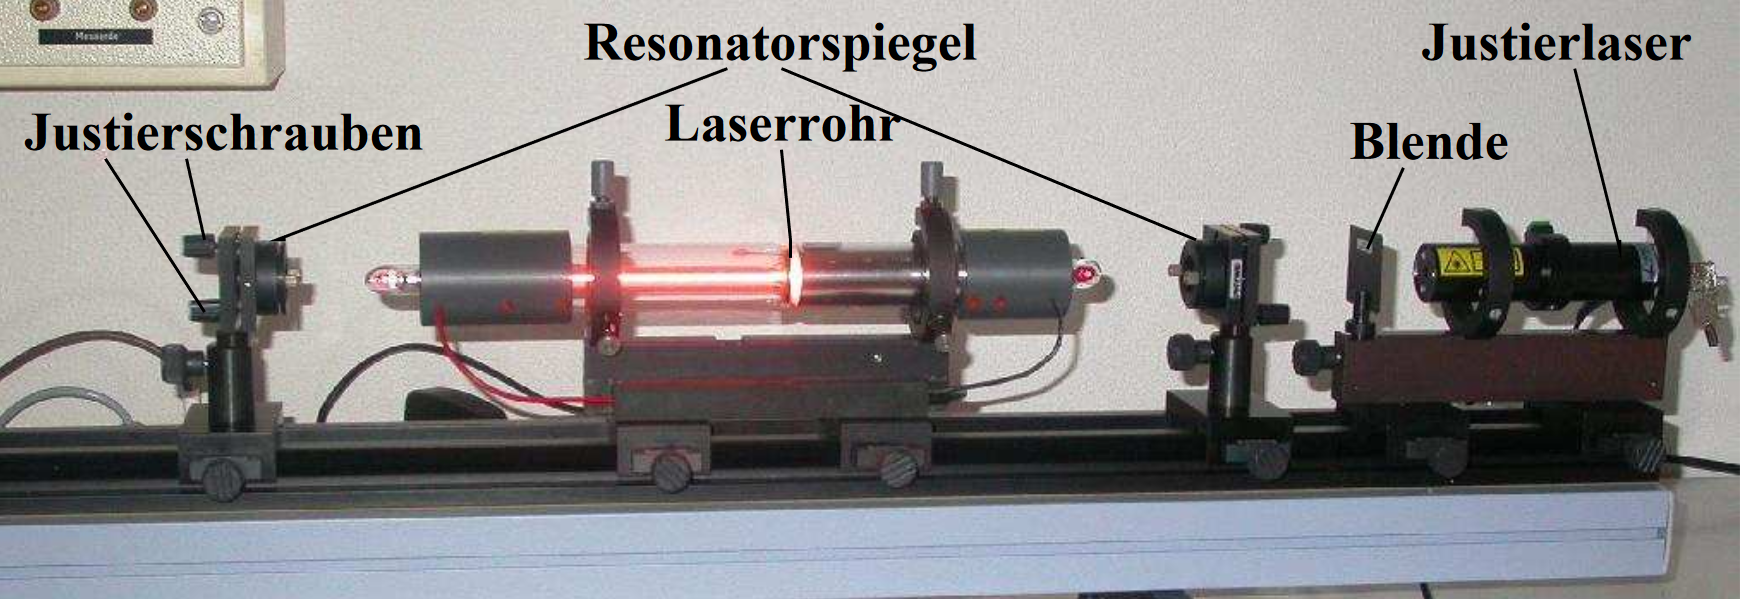
\includegraphics[width=\linewidth-30pt,height=\textheight-30pt,keepaspectratio]{content/images/aufbau.png}
\caption{Schematischer Aufbau des Prismenspektralapparates \cite{V402}.}
\label{fig:aufbau}
\end{figure}

\noindent Der Prismenspektralapparat besteht aus wie in Abbildung \ref{fig:aufbau} zu sehen im wesentlichen aus einem festen Kollimatorrohr, einem Glasprisma, welches auf dem Drehtisch eines Goniometers befestigt ist, sowie einem schwenkbaren Fernrohr. Dabei fällt das Licht einer Quecksilber-Cadmium Lampe durch den Spalt des Kollimatorrohres auf eine Sammellinse, deren Brennweite ihrem Abstand zum Spalt entspricht. Dadurch wird das Licht parallel auf das Glasprisma gelenkt und kann nach der Brechung am Prisma mit dem Fernrohr beobachtet werden. Im Fernrohr ist zur genauen Lokalisierung des Spaltbildes in der Brennebene der Objektivlinse ein Fadenkreuz angebracht.